% Copyright (c) 2014,2016 Casper Ti. Vector
% Public domain.

\chapter{比特幣監督系統實作與結果}
為了驗證和證明所提議的PBCSS用於比特幣支付收款監督的可行性和有效性,我們實施了其運行在用於商家商品管理和維護的Java應用程序的SMIMSS子系統,用於商家職員的運行在Android App上的SMCTSS以及運行在App上的用於客戶的CMPTSS。
如圖\ref{fig5}所示,SMIMSS Java應用程序可以幫助商家登錄到系統或創建一個新帳戶。 授權商戶成功登錄系統後,商家可以插入或更新產品列表,如圖\ref{fig6}所示。實施的SMIMSS Java應用程序執行前面部分中所述的功能。
%%%%%%放入fig5
\begin{figure}[h]
	\centering
	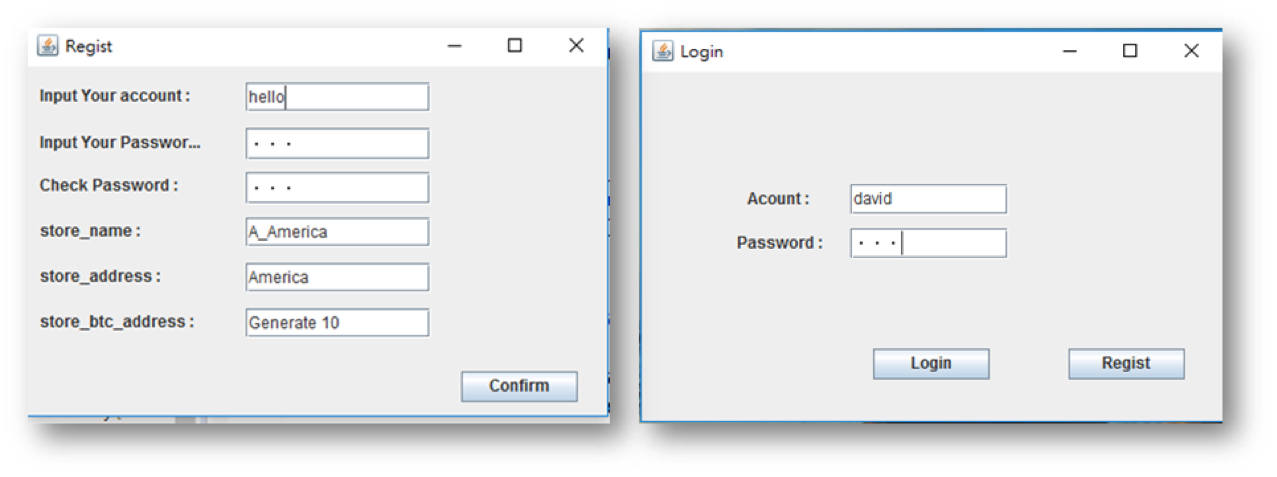
\includegraphics[width = 0.9\textwidth]{fig5.png}
	\caption{fig5}\label{fig5}
\end{figure}
%%%%%%放入fig6
\begin{figure}[h]
	\centering
	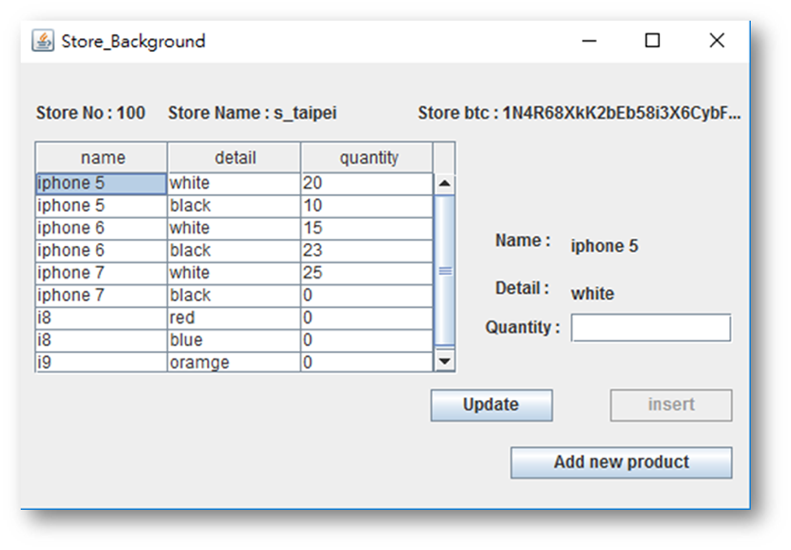
\includegraphics[width = 0.6\textwidth]{fig6.png}
	\caption{fig6}\label{fig6}
\end{figure}

商戶的產品信息包括RFID標籤通過SMIMSS存儲到雲端數據庫中後,商戶店員可以使用我們實現的SMCTSS安卓應用,啟用NFC監聽器,從購物車中的客戶購買產品中讀取RFID標籤信息。 在如圖\ref{fig7}所示的第一項活動中,商家職員必須登錄才能獲得授權訪問SMCTSS功能。 然後,在第二項活動中,SMCTSS應用程序可以通過使用SMIMSS中應用的雲數據庫檢查產品RFID標籤信息並將其展示給客戶,從而將掃描的產品列入購物車。 在圖\ref{fig7}的第三項活動中,顧客可以要求店員取消購買物品以確認最終購買。 最後,SMCTSS應用程序將自動使用比特幣測試網絡幫助店員確認發布此數字貨幣交易的收款人地址,如圖\ref{fig7}的第4項活動所示。    
%%%%%%放入fig7
\begin{figure}[h]
	\centering
	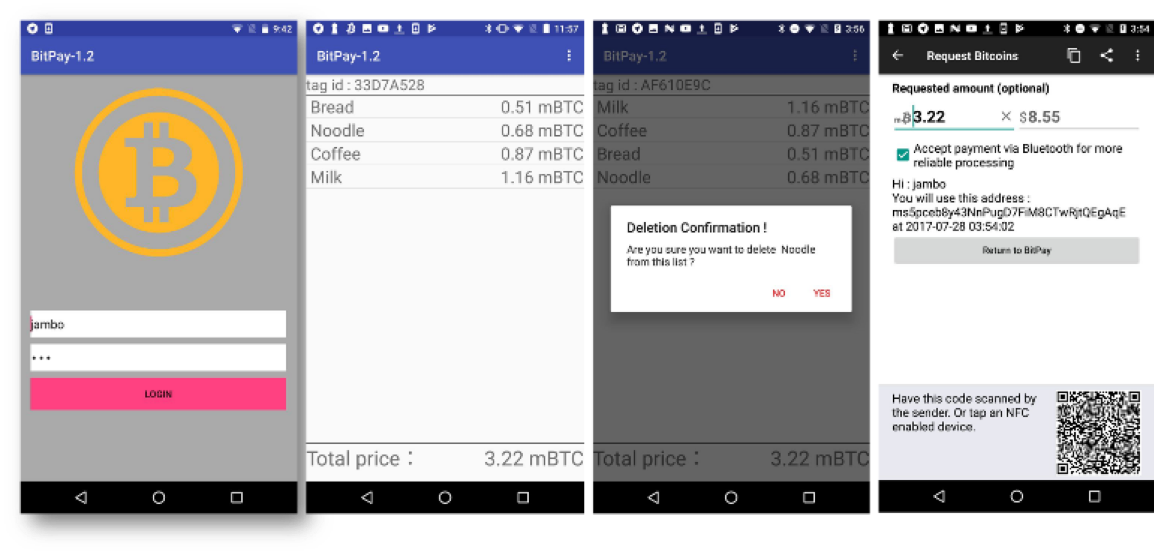
\includegraphics[width = 1\textwidth]{fig7.png}
	\caption{fig7}\label{fig7}
\end{figure}
同時,客戶將使用與SMCTSS App相對應的CMPTSS Android App通過比特幣數字貨幣完成採購產品交易。 如圖\ref{fig8}所示,第一個活動表示顧客確認購買產品創建交易數據庫的交易清單,第二個活動顯示包括金額和付款人比特幣地址在內的付款確認,第三個活動顯示交易歷史記錄 的交易作為買方甚至是賣方,最後在第四項活動中顯示了單筆交易的詳細採購產品的發票。    
%%%%%%放入fig8
\begin{figure}[h]
	\centering
	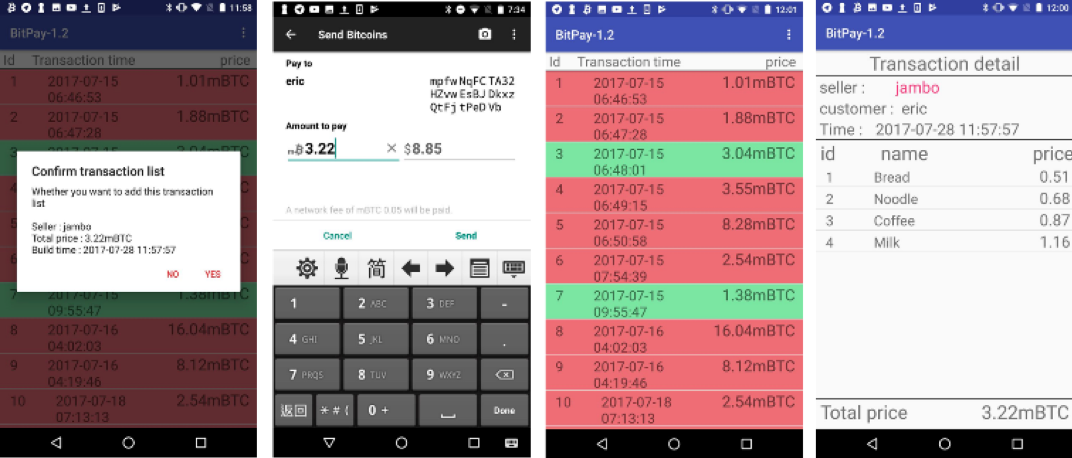
\includegraphics[width = 1\textwidth]{fig8.png}
	\caption{fig8}\label{fig8}
\end{figure}

根據比特幣點對點架構,儘管客戶和商店之間的交易細節已經快速存儲到雲數據庫,但官方確認交易與當前比特幣區塊鏈的交易通常需要更長的時間,因為需要確保確認的數量在交易廣播比特幣P2P網絡並存儲到緩存池後,反對雙重支出。
因此,為了驗證我們提出的BPCSS不會通過使用比特幣等數字貨幣影響交易完成時間,我們在我們的Testnet實驗中連續記錄了30筆交易信息。同時,我們首先使用區塊鏈工具,如圖9的第一張快照所示,其次使用Testnet按順序進行30個比特幣交易,如圖9的中間快照所示,最後30個交易完成時間全部記錄在區塊鏈中探險家。實驗結果表明,實驗中的所有交易都在3秒鐘左右(平均2.97秒,標準差小於1秒)發送到比特幣網絡緩存池,平均交易完成時間在比特幣區塊鏈中確認為522.33秒(小於9分鐘),標準差大約為339秒。比特幣測試網上的初步實驗結果表明,我們提出的BPCSS可以經濟有效地執行區塊鏈支付收款監督。    
